%%% DataMCSamples %%%
\label{ch:exp_methods}
%%%This section contains information about the various data and Monte Carlo samples used in this analysis.

\section{Data Samples}
\label{sec:data_sample}

%%%
The semileptonic VBS analysis is based on proton-proton (\pp) collision data collected from 2015 to 2018, amounting to an integrated luminosity of \intLumi\,\ifb. The overall uncertainty for the integrated luminosity, measured at 1.7\%\cite{ATLAS-CONF-2019-021}, was determined using the LUCID-2 (LUminosity Cherenkov Integrating Detector)~\cite{Avoni:2633501} for primary luminosity measurements.
Table~\ref{tab:intLumi} summarizes the integrated luminosity used in this analysis.


\begin{table}[htb!p]
\begin{center}
\caption{Integrated luminosity data used in the semileptonic VBS analysis.}
\label{tab:intLumi}
\begin{tabular}{|l|c|}
\hline
Year & $\mathcal{L}$ [\ifb] \\
\hline\hline
2015 & 3.21 \\
\hline
2016 & 32.88 \\
\hline
2017 & 44.31 \\
\hline
2018 & 58.45 \\
\hline\hline
total & $139.0 \pm 2.4$ \\
\hline
\end{tabular}
\end{center}
\end{table}



\section{Monte Carlo Simulated Samples}
\label{sec:mc_sample}
%Lists of MC samples for both the SM background and EW signal processes signals are summarized in appendix \ref{app:samplelist}.

Monte Carlo (MC) simulations are integral to nearly all stages of the analysis workflow. These simulations are essential for background modeling, signal acceptance evaluation, event selection optimization, systematic uncertainty estimation, and statistical analysis.
The MC samples are generated with ATLAS-approved settings.
The EvtGen v1.2.0 program~\cite{Lange:2001uf} simulates bottom and charm hadron decays. 
To account for pileup, additional $pp$ collisions are simulated using \textsc{Pythia} 8.186\cite{Sjostrand:2008vc} and integrated into all MC events. 
The samples undergo a comprehensive simulation of the ATLAS detector\cite{SOFT-2010-01} using \textsc{GEANT4}\cite{Agostinelli:2002hh}.
All simulated events are processed using the same trigger and reconstruction algorithms as the collected data.
Appendix \ref{app:samplelist} summarizes the MC samples for SM background and EW signal processes.



\subsubsection{Background processes}
The $V$ ($W/Z$) + jets events are simulated with Sherpa 2.2.1~\cite{Gleisberg:2008ta} and normalzied to the NNLO cross sections. 
Up to 2 partons at NLO and 4 partons at LO are considered using Comix~\cite{Gleisberg:2008fv} and OpenLoops~\cite{Cascioli:2011va} for matrix element calculations, integrated with the Sherpa parton shower~\cite{Schumann:2007mg} using the ME+PS@NLO prescription~\cite{Hoeche:2012yf}. 
These simulations use the NNPDF3.0NNLO PDF set alongside specific tuning~\cite{Ball_2015}. 
%% $W$/$Z$ + jets samples are normalzied to the NNLO cross sections.

As alternative \Vjets MC samples for the analysis, QCD $V$+jets production was simulated using \MGNLO[2.2.2]~\cite{Alwall:2014hca} with LO-accurate matrix elements (ME) featuring up to four final-state partons. 
These ME calculations utilized the \NNPDF[3.0nlo] PDF set~\cite{Ball:2014uwa} for $H_\text{T}$-sliced and the \NNPDF[2.3lo] set~\cite{Ball:2012cx} for $N_\text{parton}$-sliced events. 
The events were then interfaced with \PYTHIA[8.186]~\cite{Sjostrand:2007gs} to simulate the parton shower, hadronization, and the underlying event dynamics.
The CKKW-L merging procedure~\cite{Lonnblad:2001iq,Lonnblad:2011xx} was applied to eliminate overlap between matrix element calculations and parton shower emissions.
The A14 tune of \PYTHIA[8]~\cite{ATL-PHYS-PUB-2014-021}, in conjunction with the \NNPDF[2.3lo] PDF set~\cite{Ball:2012cx}, was used. 
Decays of bottom and charm hadrons were handled by \EVTGEN[1.2.0]~\cite{Lange:2001uf}. 
Although not the nominal samples, these $V$+jets samples were normalized to NNLO predictions~\cite{Anastasiou:2003ds} and served to derive modeling uncertainties for the \Vjets background.

The \ttbar and single-top events are generated using Powheg-Box~\cite{Alioli:2010xd} and NNPDF3.0NLO PDF sets~\cite{Ball:2014uwa} for matrix element calculations, ensuring top quark spin correlations are preserved. 
Specifically, t-channel top quarks are decayed with MadSpin~\cite{Artoisenet:2012st}. 
\textsc{Pythia}8.230 simulates the parton shower, fragmentation, and underlying event dynamics using the A14 tune set~\cite{ATL-PHYS-PUB-2014-021}, with the top quark mass set at $172.5\gev$. 
The cross sections for \ttbar and single-top processes are calculated with NNLO precision in QCD, which includes the re-summation of next-to-next-to-leading logarithmic (NNLL) soft gluon terms~\cite{Czakon:2011xx,Kidonakis:2011wy,Kidonakis:2010tc,Kidonakis:2010ux}.
The \textsc{Hdamp} parameter, which regulates high-\pt\ radiation in \textsc{Powheg}, is set to $1.5m_{t}$ to ensure good data/MC agreements in the high-\pt\ region\cite{ATL-PHYS-PUB-2016-020}.

The $q\bar{q}$-induced diboson processes ($WW$, $WZ$, and $ZZ$) are simulated using \SHERPA[2.2.1] or 2.2.2~\cite{Bothmann:2019yzt}, as per the specific process. 
These simulations incorporate off-shell effects and, where relevant, Higgs boson contributions. 
The matrix elements are calculated with NLO QCD accuracy for up to one additional parton and LO accuracy for up to three additional partons.

Loop-induced $gg \to VV$ processes were simulated using LO-accurate matrix elements with up to one additional parton emission, covering both fully leptonic and semileptonic final states. These calculations were harmonized and combined with the \SHERPA parton shower via Catani--Seymour dipole factorisation~\cite{Gleisberg:2008fv,Schumann:2007mg}, following the MEPS@NLO prescription~\cite{Hoeche:2011fd,Hoeche:2012yf,Catani:2001cc,Hoeche:2009rj}.

QCD diboson production from $gg$ initial states is excluded from the final results due to its significantly smaller expected cross section compared to the baseline QCD $VV$ production; their impact has been evaluated and found to be negligible.


\subsubsection{Signal SM EW VV+jj processes}
\label{sec:mc_sample_ewvvjj}

The EWK $VV+jj$ production is simulated with MadGraph5\_aMC@NLO v2.3.3~\cite{Alwall:2014hca} and \PYTHIA8~\cite{Sjostrand:2007gs} for fragmentation, using the \textsc{NNPDF30NLO} PDF set~\cite{Ball:2012cx}. 
The samples feature two on-shell $V$ bosons: one decaying leptonically ($Z \to \ell\ell$ where $\ell = e, \mu$; $Z \to \nu\nu$; $W \to \ell \nu$ with $\ell= e, \mu, \tau$), and the other hadronically. 
Both $W^{+}$ and $W^{-}$ decays are included, and for $WWjj$, all charge combinations ($W^{+}W^{+}$, $W^{+}W^{-}$, and $W^{-}W^{-}$) are considered. 
Table~\ref{tab:VBS_sig_samples} details the EWK $VV+jj$ samples used in this analysis.
In these samples, we account for all purely-electroweak tree-level diagrams of order $\mathcal{O}(\alpha_{EW}^6)$ that contribute to the final states. This includes both VBS diagrams and non-VBS electroweak diagrams. Detailed examples of these diagrams have been previously discussed and are showcased in Figures~\ref{fig:feynmanVBS} and \ref{fig:feynmanEWKnonVBS}, as found in Section~\ref{section:Vector_Boson_Scattering}.


For EWK $WW+jj$ production, the non-VBS electroweak $t\bar{t}$ diagrams, as depicted in Fig.~\ref{fig:feynmanEWKnonVBS}(e) and (f), could significantly contribute. This potential issue is effectively mitigated through the use of a $b$-veto. Despite this mitigation, the contribution from the non-VBS $tZb$ process, illustrated in Fig.~\ref{fig:feynmantZb}, remains considerable. To address this, a cut was implemented near the reconstructed top mass, effectively reducing its impact, as detailed in Table~\ref{tab:1lep_resolved}.

Diagrams that feature both electroweak and QCD vertices, with an order of $\mathcal{O}(\alpha_{EW}^{4} \alpha_s^{2})$, are not included in these signal samples and are not part of the signal definition.
Examples of such diagrams are depicted in Fig.~\ref{fig:feynmanQCD}. These processes, unaffected by aQGCs, are considered part of the background, including $t\bar{t}$, single-top, and diboson events.

%%%fixed eff
\begin{table}[!htbp]
\begin{center}
\small
\caption{List of VBS samples used in the analysis.}
\begin{tabularx}{\textwidth}{|c|c|X|X|X|c|c|c|}
\hline
Process & DSID & Events - mc16a & Events - mc16d & Events - mc16e & Filter efficiency & cross-section~(pb) \\
\hline

$\Wlv\Wqq jj, b-veto$    & 364848   &   1958000 &  2296000 & 3320000 & 0.17465  &  1.9994  \\
$\Wlv\Wqq jj, b-filter$  & 364849   &   1996000 &  2400000 & 3388000 & 0.83126  &  1.9777  \\
$\Wlv\Zqq jj$            & 364850   &   1994000 &  2394000 & 3392000 & 1.0  &  0.2571  \\
$\Zvv\Wqq jj$            & 364851   &   1986000 &  2394000 & 3356000 & 1.0  &  0.15532  \\
$\Zll\Wqq jj$            & 364852   &   1996000 &  2374000 & 3390000 & 1.0  &  0.045609  \\
$\Zvv\Zqq jj$            & 364853   &   1998000 &  2396000 & 3390000 & 1.0  &  0.032238  \\
$\Zll\Zqq jj$            & 364854   &   1990000 &  2388000 & 3396000 & 1.0  &  0.0096553  \\

\hline
\end{tabularx}
\label{tab:VBS_sig_samples}
\end{center}
\end{table}

%% feynman diagram, tZb
\begin{figure}[tbp]
\begin{center}
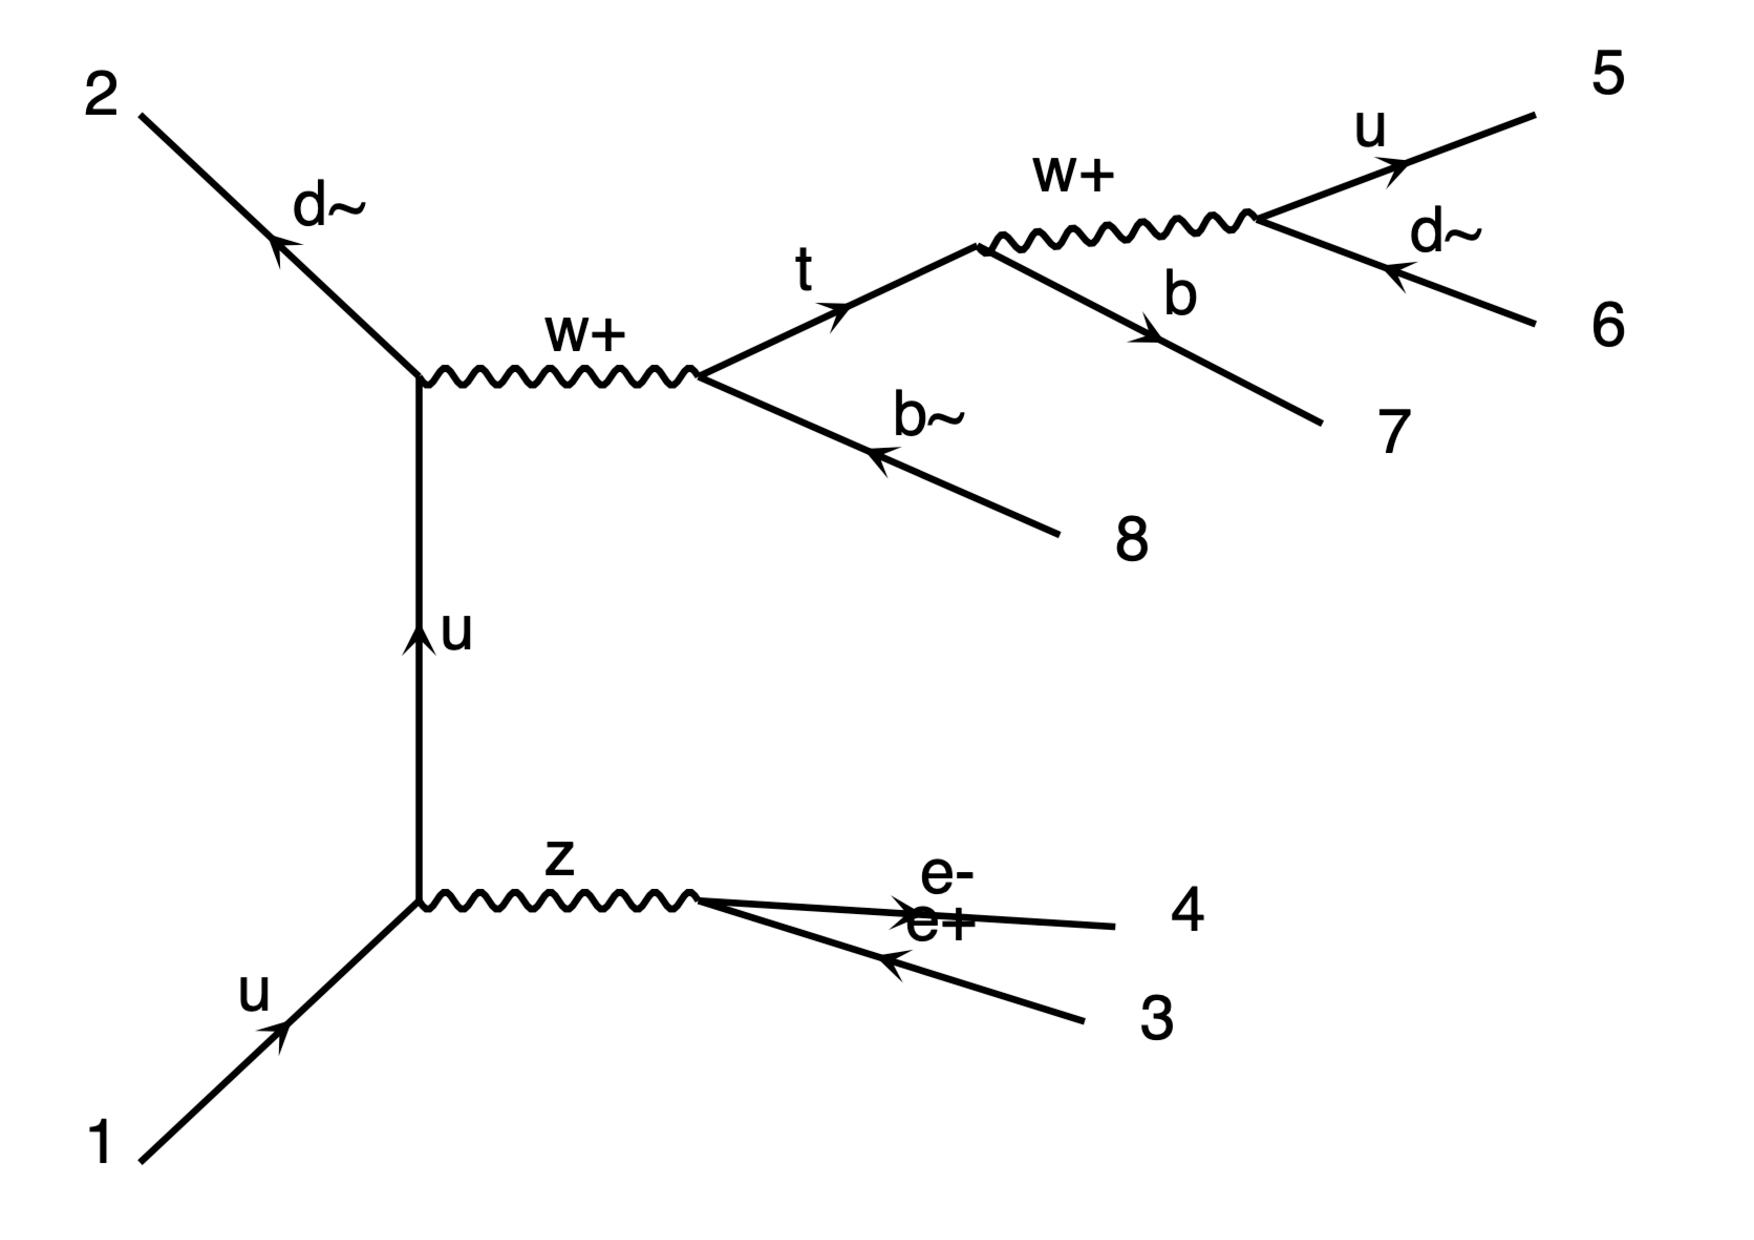
\includegraphics[width=0.35\textwidth]{figures/samples/feynEWKnonVBStZb.pdf}
\caption{
The example of the tZb diagram, which included in non-VBS $\mathcal{O}(\alpha_{EW}^6)$ diagrams. 
}
\label{fig:feynmantZb}
\end{center}
\end{figure}
%% feynman diagrams, QCD
%
\begin{figure}[tbp]
\begin{center}
\subfloat[]{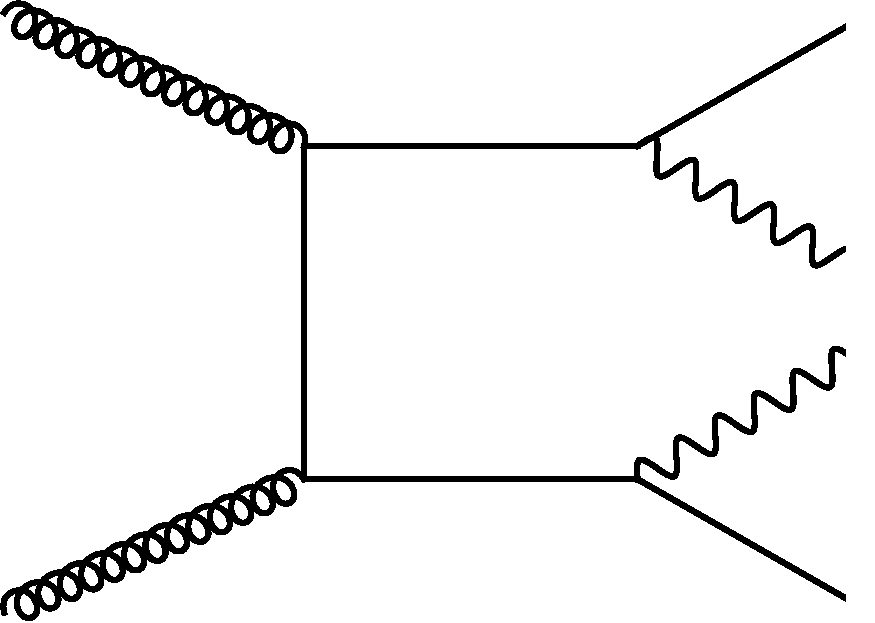
\includegraphics[width=0.3\textwidth]{figures/samples/feynQCD3.pdf}}
\subfloat[]{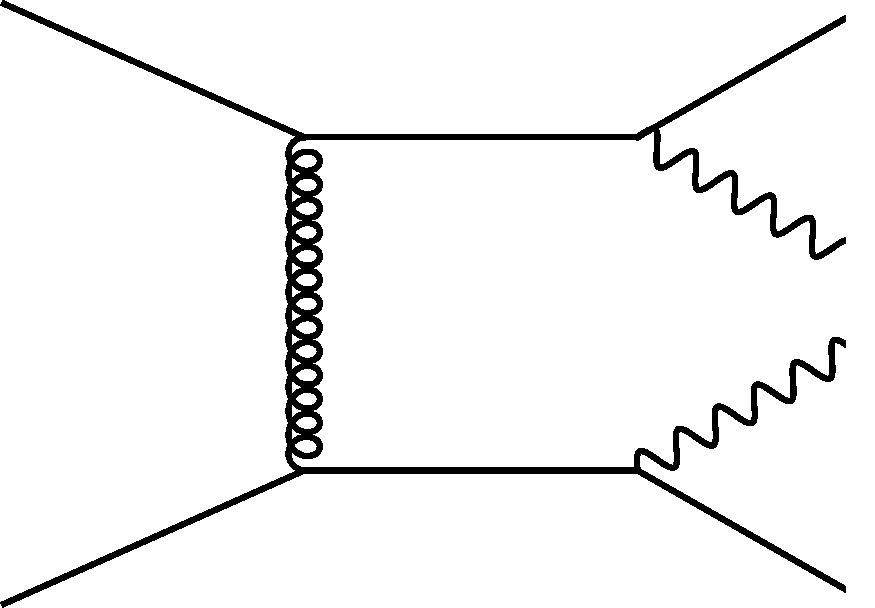
\includegraphics[width=0.3\textwidth]{figures/samples/feynQCD4.pdf}}
\subfloat[]{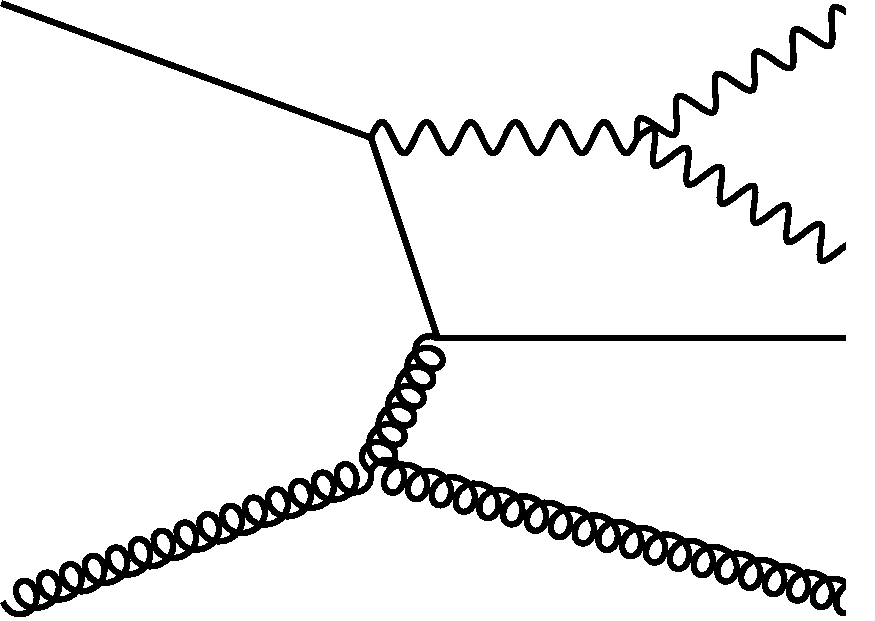
\includegraphics[width=0.3\textwidth]{figures/samples/feynQCD5.pdf}}\\
\subfloat[]{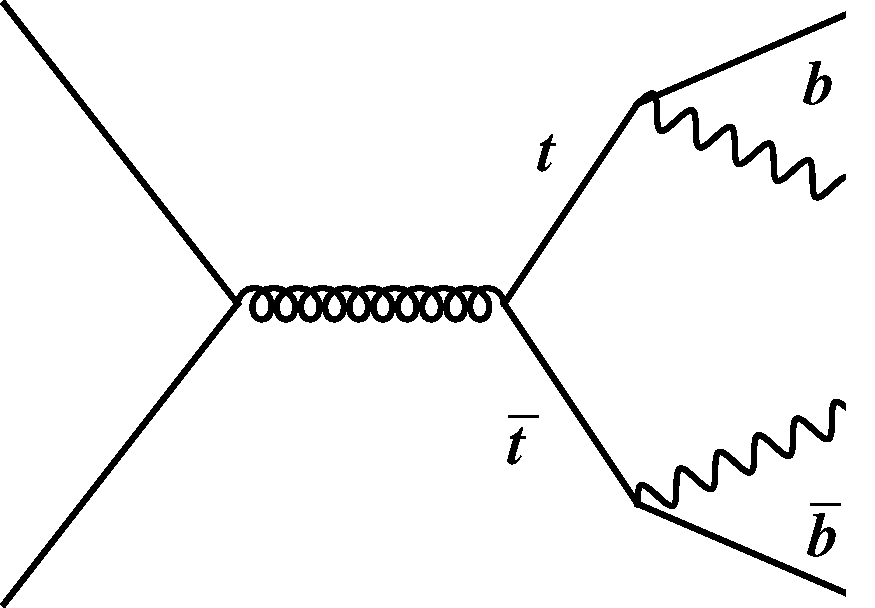
\includegraphics[width=0.3\textwidth]{figures/samples/feynQCD1.pdf}}
\subfloat[]{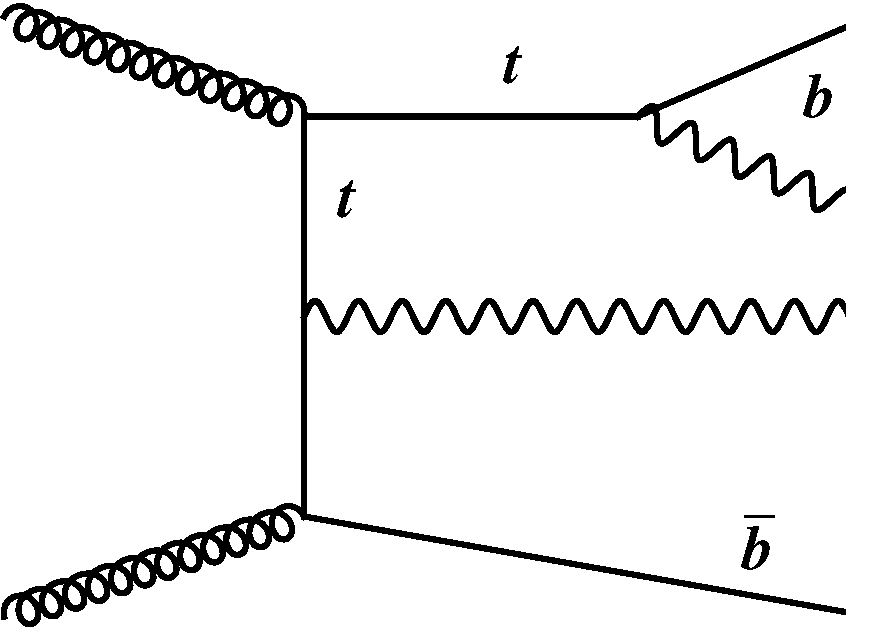
\includegraphics[width=0.3\textwidth]{figures/samples/feynQCD2.pdf}}
\caption{
Examples of $\mathcal{O}(\alpha_{EW}^4 \alpha_{S}^2)$ diagrams that lead to the $VV$+2 parton final state. 
}
\label{fig:feynmanQCD}
\end{center}
\end{figure}

\clearpage
\subsubsection{Signal aQGC processes}
\label{subsec:agc_sample}

As discussed in Section~\ref{Anomalous_Quartic_Gauge_Couplings}, the Eboli model is used to model potential aQGC effects in the VBS process. This model includes 21 D-8 operators, 19 of which can alter the semileptonic VBS final state.
The matrix element for a SM process, incorporating new contributions from EFT, can be expressed as follows:
\begin{equation}
  |A_{\text{SM}} + c_i A_i|^2 = |A_{\text{SM}}|^2 + \sum\limits_i c_i^2 |A_i|^2 + \sum\limits_i 2 c_i \mathrm{Re}(A_{\text{SM}}^\star A_i) + \sum\limits_{i \neq j} c_i c_j \mathrm{Re}(A_i^\star A_j)
\end{equation}
Here, $|A_{\text{SM}}|^2$ denotes the squared matrix element for the SM process, $|A_i|^2$ represents the squared matrix element for pure EFT contributions, $2 \mathrm{Re}(A_{\text{SM}}^\star A_i)$ is the interference between the SM and EFT contributions, and $\mathrm{Re}(A_i^\star A_j)$ is the interference among different EFT contributions. This formulation allows for a detailed breakdown of the process, which can be useful with the matrix-element decomposition method available in recent versions of MadGraph5\_aMC@NLO, enabling the specific generation of each term individually.

To model the Eboli D-8 EFT processes, we generate a series of samples for each operator \(A_i\) at varying coefficient values (\(c_i\)). We utilize MadGraph5\_aMC@NLO version 2.7.2 for these simulations at leading order (LO), incorporating the NNPDF30LO parton distribution function (PDF) set~\cite{Ball:2012cx}, and Pythia 8.244~\cite{Sjostrand:2007gs} for fragmentation processes. The matrix element calculation results in two on-shell \(W/Z\) bosons, which are subsequently decayed using \textsc{MadSpin}~\cite{Artoisenet:2012st} to represent the leptonic and hadronic decay channels. Due to the matrix-element weighting requirements, simulations for each weak isospin state of the boson (e.g., \(W^+W^-\), \(W^+W^+\), \(W^-W^-\), \(W^+Z\), \(W^-Z\), \(ZZ\)) are conducted separately.


\section{Derivation and CxAOD framework}
\label{subsec:DxAOD_and_CxAOD}
%Some technical details on the derivations and analysis framework are described in this section.
For the 1-lepton analysis, we employ the \texttt{HIGG5D2} derivation, which is produced by Athena's derivation framework. This framework consists of tools, algorithms, and Python scripts designed to produce analysis data formats known as derived AODs (DAODs), essential for initiating most analyses. 
DAODs streamline the analysis process by providing a refined dataset, having undergone preliminary selection cuts to minimize data size. These initial cuts are listed in Table~\ref{tab:presel_DxAOD}. Typically, DAODs are generated by a central production team, meaning individual researchers usually engage with the framework directly only for testing purposes on a smaller scale.

\begin{table}[t]
\caption{Pre-selections in the derivation framework for data size reduction. 
$N_j$, $N_J^{\textrm{TCC}}$, and $N_J^{\textrm{LCTopo}}$ represent the counts of different types of jets.} 
\label{tab:presel_DxAOD}
\begin{center}
\resizebox{0.7\textwidth}{!}{
\begin{tabular}{|l|c|}
\hline
\multicolumn{2}{|c|}{ HIGG5D2 ($\ell\nu qq$) } \\
\hline
Trigger & \textit{OR} of all single-lepton and \met triggers \\
\hline
Number of leptons   & $\geq 1$ \\
\hspace{1cm}(lepton \pt)        & $> 20\,\GeV$ \\
\hspace{1cm}(electron quality) & \texttt{DFCommonLHLoose} \\
\hspace{1cm}(muon quality)      & \texttt{DFCommonGoodMuon} \\
\hline
Number of jets      & $N_j \geq 1$ or $N_J^{\textrm{TCC}} + N_{J}^{\textrm{LCTopo}} \geq 1$ \\
\hline
\end{tabular}
}
\end{center}
\end{table}

We use the common analysis \texttt{CxAOD} framework (version \texttt{r33-12}) for this analysis.
The \texttt{CxAOD} framework is used to define physics objects, adhere to all CP recommendations for them, and apply pre-selection cuts.
These procedures and definitions are detailed in Sections~\ref{chap:objects_def} and \ref{subsec:event_preselection}, respectively.
The CP recommendations are providede by the combined performance (CP) groups for use in analysis.
